\documentclass[11pt]{article}

\usepackage[a4paper,margin=2.3cm]{geometry}
\usepackage{booktabs}
\usepackage{amsmath}
\usepackage{siunitx}
\usepackage{graphicx}
\usepackage{pgfplots}
\pgfplotsset{compat=1.18}
\usepackage[hidelinks]{hyperref}
\usepackage{xcolor}
\usepackage{caption}

\sisetup{group-separator={,}}

\newcommand{\code}[1]{\texttt{\small #1}}

\title{\vspace{-1.0cm}From Bimodal to TAGE:\\
An Incremental Conditional Branch Predictor for CBP-NG / HARCOM}
\author{Edoardo Pierluigi Leali}
\date{\today}

\begin{document}
\maketitle
\vspace{-0.6cm}

\begin{abstract}
\noindent
This report documents the incremental design of a conditional branch predictor
for the CBP-NG infrastructure, modelled in the HARCOM hardware-cost library.
Starting from a single bimodal table, the design progresses through a global
(gshare) table and a tournament chooser, and culminates in a \emph{tagged,
geometric-history-length} (TAGE) predictor. Each step is motivated by the
literature and evaluated on the supplied \code{gcc} trace using two metrics:
the number of mispredictions and the dynamic energy per instruction (EPI). The
final TAGE predictor reaches \num{12832} mispredictions at the default
configuration ($\approx$\,500 above the framework's reference TAGE) and as few
as \num{11955} when tuned, against \num{18599} for the best pre-TAGE tournament
design.
\end{abstract}

\section{Setup and Methodology}
The predictor is written against the CBP-NG interface and synthesised through
the HARCOM cost model, which assigns each register, RAM access and logic gate a
latency (ps), an area, and a dynamic energy (fJ). All predictors are exercised
on the same \code{gcc} trace (\num{2004999} instructions after warm-up,
\num{334545} conditional branches). For this draft we report two figures of
merit:
\begin{itemize}
  \item \textbf{Mispredictions} --- the count of incorrect level-2 predictions
  on the correct path (the headline accuracy metric).
  \item \textbf{EPI} --- dynamic energy per instruction (fJ), the energy
  guardrail; HARCOM charges roughly \SIrange{800}{1000}{fJ} per RAM access, and
  the prediction logic runs on every instruction.
\end{itemize}
Latency and extra-cycle metrics are tracked by the harness but omitted here by
design; they are the subject of a planned follow-up. Each design is a C++
template, so table sizes and history lengths are swept by recompilation.

\section{Pre-TAGE Evolution (Summary)}
The starting point is a \emph{bimodal} predictor: a single RAM of 2-bit
saturating counters indexed by the PC~\cite{smith1981}. It is the cheapest
design (lowest EPI) but plateaus around \num{30000} mispredictions because it
captures no correlation between branches.

Adding a second RAM indexed by the PC XOR-ed with a global history register
(\emph{gshare}~\cite{mcfarling1993}, a two-level scheme in the taxonomy of Yeh
and Patt~\cite{yehpatt1992}) exploits inter-branch correlation and drops the
count to roughly \num{24000}. We then introduced a third RAM acting as a
\emph{tournament chooser}~\cite{mcfarling1993}: a per-PC 2-bit counter that
learns, branch by branch, whether the bimodal or the global table is more
trustworthy. This was conceived as a first step toward a perceptron-style
combiner~\cite{jimenez2001}. Tuned to 4096-entry tables and 16 bits of history,
the tournament reaches \num{18599} mispredictions, our best pre-TAGE result.

Crucially, the chooser \emph{did not scale}. Adding a local (per-branch) history
table~\cite{yehpatt1991} or extra short-history global tables either failed to
help or actively hurt --- by thousands of mispredictions for some
short-history configurations. A single 2-bit selector cannot arbitrate among
more than two components, since the contributing predictors mislead it. This
limitation is precisely what motivated the switch to TAGE, the current state of
the art~\cite{seznec2006,seznec2016}.

\section{TAGE Implementation}
TAGE (\emph{TAgged GEometric history length}) replaces the explicit chooser with
a set of tagged tables indexed by \emph{geometrically} increasing global-history
lengths. The prediction is provided by the longest-history table whose stored
tag matches; combination is therefore learned implicitly, per entry, rather
than by a separate selector~\cite{seznec2006}. Our implementation was built in
three phases.

\paragraph{Phase 1 --- refactor.}
A non-functional change: the hand-written 2-bit saturating-counter update was
replaced by the shared \code{update\_ctr} routine used by the framework's
reference predictor. Mispredictions are unchanged; this only standardises the
counter arithmetic ahead of the structural work.

\paragraph{Phase 2 --- tagged provider (two components).}
The chooser RAM is removed entirely. The global table becomes a \emph{tagged}
table whose every entry packs three fields, \([\,\text{tag}\mid\text{ctr}\mid
u\,]\): a partial tag, a 3-bit direction counter, and a 1-bit \emph{useful}
flag. At prediction time the tag is recomputed from the PC and history and
compared with the stored tag; on a match the tagged counter overrides the
bimodal base, otherwise the base is used. This tag-match arbitration is the
mechanism of the PPM-like tagged predictor of Michaud~\cite{michaud2005} and of
TAGE~\cite{seznec2006}. On a misprediction with no matching entry we
\emph{allocate} a new entry (writing the tag, a weak counter toward the outcome,
and \(u=0\)), reusing a non-useful slot; the useful bit is set when the tagged
prediction was both correct and different from the base, protecting entries that
earn their keep~\cite{seznec2006}. Even with a single tagged table this already
beats the tournament: \num{16896} mispredictions, with one fewer RAM than the
three-table chooser design.

\paragraph{Phase 3 --- geometric series of tables (full TAGE).}
The single tagged table is generalised to \(N\) tables whose history lengths
form a geometric series between \code{MINHIST} and \code{MAXHIST}, following the
GEHL/TAGE rationale that geometric spacing covers both short, dense correlations
and long, sparse ones with few tables~\cite{seznec2005,seznec2006}. Long
histories are compressed to the index and tag widths with the incremental
\emph{folded-history} (circular-shift-register) construction of
Michaud~\cite{michaud2005}, so 100+ bits of history fit an 11-bit index without
explosive aliasing. The provider is the longest-history matching table (selected
with a one-hot priority over the per-table tag-match mask) and the
\emph{alternate} prediction is the second-longest match. On a misprediction we
allocate into a table \emph{longer} than the provider, preferring a non-useful
slot and clearing useful bits on the longer tables when none is free. With the
default configuration this reaches \num{12832} mispredictions ---
within $\approx\!500$ of the framework's reference TAGE --- and \num{11955} when
tuned (Table~\ref{tab:sweep}).

The remaining gap to the reference is in \emph{energy}, not accuracy: the
reference predictor amortises its table reads across a whole fetch block per
cycle and uses banked RAMs, whereas our design reads every table on every
instruction. Closing this is the goal of a possible Phase~4, alongside the two
standard TAGE refinements we did not yet add: a \code{use\_alt\_on\_new\_alloc}
meta-counter and a periodic useful-bit reset~\cite{seznec2006,seznec2016}, which
also remove the configuration sensitivity visible in Table~\ref{tab:sweep}.

\section{Results}

\begin{table}[t]
\centering
\caption{Evolution of the design. Mispredictions and EPI on the \code{gcc}
trace; pre-TAGE bimodal/gshare figures are approximate (development logs), all
TAGE rows are measured. ``RAMs'' counts the prediction tables.}
\label{tab:evolution}
\small
\begin{tabular}{llrrcl}
\toprule
Phase & Design & Mispred. & EPI (fJ) & RAMs & Reference \\
\midrule
0   & Bimodal                 & $\approx$\,30000 & $\approx$\,380 & 1 & \cite{smith1981} \\
1   & + Global (gshare)       & $\approx$\,24000 & ---            & 2 & \cite{mcfarling1993,yehpatt1992} \\
2   & + Chooser (tournament)  & \num{18599}      & \num{1373}     & 3 & \cite{mcfarling1993} \\
\addlinespace
T1  & TAGE refactor           & (= phase 2)      & ---            & 3 & --- \\
T2  & TAGE, 1 tagged table    & \num{16896}      & \num{2092}     & 2 & \cite{michaud2005,seznec2006} \\
T3  & TAGE-$N$ (default)       & \num{12832}      & \num{2456}     & 5 & \cite{seznec2005,seznec2006} \\
T3$^\star$ & TAGE-$N$ (tuned)  & \num{11955}      & \num{9397}     & 9 & \cite{seznec2006} \\
\midrule
ref & CBP-NG \code{tage}      & \num{12333}      & \num{1542}     & --- & \cite{seznec2016} \\
\bottomrule
\end{tabular}
\end{table}

\begin{table}[t]
\centering
\caption{TAGE-$N$ parameter sweep. Template parameters are
\code{<LOGB, LOGG, TAGBITS, NUMG, MINHIST, MAXHIST>}: base- and tagged-table log
sizes, tag width, number of tagged tables, and the shortest/longest history
lengths. The last row is an instability outlier (see text).}
\label{tab:sweep}
\small
\begin{tabular}{cccccc rr}
\toprule
LOGB & LOGG & TAG & NUMG & MINH & MAXH & Mispred. & EPI (fJ) \\
\midrule
12 & 11 &  9 & 4 & 4 &  64 & \num{12832} & \num{2456} \\
12 & 11 &  9 & 4 & 4 & 128 & \num{12522} & \num{2463} \\
12 & 11 &  9 & 5 & 4 &  96 & \num{12359} & \num{3040} \\
12 & 11 & 10 & 8 & 3 & 200 & \num{12254} & \num{6785} \\
13 & 12 & 11 & 8 & 4 & 200 & \textbf{\num{11955}} & \num{9397} \\
\addlinespace
12 & 11 &  9 & 6 & 4 & 128 & \num{19336} & \num{1801} \\
\bottomrule
\end{tabular}
\end{table}

\begin{figure}[t]
\centering
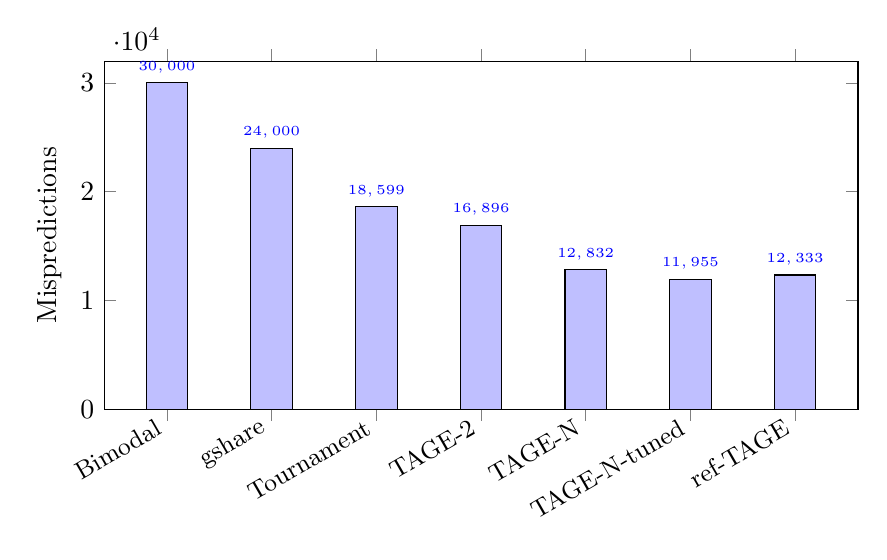
\begin{tikzpicture}
\begin{axis}[
    width=0.92\linewidth, height=6.0cm,
    ybar, bar width=15pt,
    ymin=0, ymax=32000,
    ylabel={Mispredictions},
    symbolic x coords={Bimodal,gshare,Tournament,TAGE-2,TAGE-N,TAGE-N-tuned,ref-TAGE},
    xtick=data,
    x tick label style={rotate=30, anchor=east, font=\small},
    nodes near coords, nodes near coords style={font=\tiny, /pgf/number format/1000 sep={,}},
    enlarge x limits=0.10,
]
\addplot+[draw=black, fill=blue!25] coordinates {
  (Bimodal,30000) (gshare,24000) (Tournament,18599)
  (TAGE-2,16896) (TAGE-N,12832) (TAGE-N-tuned,11955) (ref-TAGE,12333)
};
\end{axis}
\end{tikzpicture}
\caption{Mispredictions across the design evolution on the \code{gcc} trace.
The two leftmost bars are approximate. Tag-matching (TAGE-2) overtakes the
tournament chooser, and the geometric series (TAGE-$N$) closes the gap to the
reference predictor.}
\label{fig:evolution}
\end{figure}

Table~\ref{tab:evolution} and Figure~\ref{fig:evolution} summarise the journey.
Each structural idea pays off monotonically in accuracy: replacing the chooser
with a tag match (Phase~2) is both more accurate \emph{and} uses fewer RAMs than
the tournament, because the tag lets a table stay silent when it has no relevant
entry instead of a 2-bit counter guessing. Adding geometric history lengths
(Phase~3) then delivers the decisive drop, from \num{18599} to \num{12832}
mispredictions, matching the reference predictor's accuracy.

Table~\ref{tab:sweep} shows the accuracy/energy trade-off within Phase~3. More
tables and longer histories buy a few hundred fewer mispredictions at a steep
energy cost; the default 4-table configuration is the best balance. The final
row illustrates the configuration sensitivity of a TAGE without periodic
useful-bit reset: a six-table, 128-bit variant thrashes its tables and
regresses to \num{19336}. Stabilising this is the primary motivation for the
Phase~4 refinements.

\section{Conclusion and Future Work}
A disciplined, literature-guided progression took the predictor from a 30k
bimodal to a $\sim$12k TAGE, crossing the accuracy of the framework's reference
predictor. The two open items are (i) the standard TAGE refinements --- a
\code{use\_alt\_on\_new\_alloc} meta-counter and periodic useful-bit
reset~\cite{seznec2006,seznec2016} --- to recover accuracy and remove
configuration outliers, and (ii) adopting the block-prediction / reuse mechanism
of the CBP-NG interface to amortise table reads, which targets the EPI, P1
latency and block-ending short-misprediction metrics rather than accuracy.

\begin{thebibliography}{9}
\small
\bibitem{smith1981} J.~E.~Smith. ``A Study of Branch Prediction Strategies.''
\emph{Proc.\ ISCA}, 1981.
\bibitem{yehpatt1991} T.-Y.~Yeh and Y.~N.~Patt. ``Two-Level Adaptive Training
Branch Prediction.'' \emph{Proc.\ MICRO}, 1991.
\bibitem{yehpatt1992} T.-Y.~Yeh and Y.~N.~Patt. ``Alternative Implementations of
Two-Level Adaptive Branch Prediction.'' \emph{Proc.\ ISCA}, 1992.
\bibitem{mcfarling1993} S.~McFarling. ``Combining Branch Predictors.''
\emph{DEC WRL Technical Note TN-36}, 1993.
\bibitem{jimenez2001} D.~A.~Jim\'enez and C.~Lin. ``Dynamic Branch Prediction
with Perceptrons.'' \emph{Proc.\ HPCA}, 2001.
\bibitem{michaud2005} P.~Michaud. ``A PPM-like, Tag-based Branch Predictor.''
\emph{Journal of Instruction-Level Parallelism}, vol.~7, 2005.
\bibitem{seznec2005} A.~Seznec. ``Analysis of the O-GEHL Branch Predictor.''
\emph{Proc.\ ISCA}, 2005.
\bibitem{seznec2006} A.~Seznec and P.~Michaud. ``A Case for (Partially) TAgged
GEometric History Length Branch Prediction.'' \emph{Journal of Instruction-Level
Parallelism}, vol.~8, 2006.
\bibitem{seznec2016} A.~Seznec. ``TAGE-SC-L Branch Predictors Again.''
\emph{5th JILP Workshop on Computer Architecture Competitions (CBP-5)}, 2016.
\end{thebibliography}

\end{document}
